\chapter{DISCUSSION}
\label{ch:discussion}

\section{Volume Registration}

The comparison of the simulated and clinical brain rs-fMRIs using the FD and DVARS metrics showed little difference with respect to reducing the positional and signal effects of motion between pairs of subsequent time points. In the set of placenta images, both registration types improved the number of image volumes meeting the DVARS thresholds. These metrics were not considered sufficient for examining the effects of registration on patient motion, so the similarity matrices were employed. For the simulated data cohort, the minimum values and quartiles of the distributions of the Dice and MI matrices increased more for the DAG-registered sequences than for the original sequences. The changes in the similarity matrix distributions was comparable overall for the clinical images.

An additional analysis was performed for the simulated images. The goal of this analysis was to evaluate the effects of volume registration on the brain signal present in an rs-fMRI image. It was found that the DAG-registered sequences had correct voxel classifications when compared to the DMN ROI than the traditional registration did. 

This finding has interesting potential. Subject motion during rs-MRI scans affects both the recorded position and orientation of the subject as well as the established magnetic spin gradients within the skull and the susecptibility recorded in each voxel. The primary focus of volume registration has been to reduce the positional effects of motion. Correction of the spin history effects and the susceptibility effects are considered to be a separate albeit related area of research. The results of the independent component analysis of the simulated images suggest that the DAG-based registration may contribute to the reduction of the signal-based effects of motion. It could potentially be coupled with prospective motion monitoring techniques, $B_0$ field maps, and navigator sequences to address the other half of the motion problem.

All images used in these analyses consisted of brain tissue against an empty background. The images had undergone processing to remove tissues outside the skull either using automated tools or manual segmentation. The use of manual segmentation with multiple annotators has the potential to confound the results of motion correction experiments. The segmentation process may not remove all non-brain tissue from the image. Those images would then contain brain tissue, non-brain tissue, and dark background. The registration process optimizes the alignment of values in a pair of images. In some cases, the registration reach a state where the lowest cost alignment aligns tissue in general and not specifically brain tissue. While these alignments would have the lowest cost, the would not be physically correct. This problem would be difficult to detect in the metrics extracted from the image sequence: the metrics only measure the properties of the voxel values in the sequence, not of the physiological information it contains. 

Specifically, this limitation pertains to our fetal scans. The masks generated during the segmentation process were created to be uniform across the whole sequence. However, fetal motion is highly variable. The subject may drastically change position in the middle of the scan, possibly several times. The manually created masks were developed using a software tool which allows 3D image masks to be applied to an entire 4D image sequence. The masks were required to be created to ensure the fetal brain or placenta would be inside the masked area at all times and therefore may not have removed all tissues that were not of interest.

This limitation can be resolved by incorporating computer vision principles into the anatomical aspects of image segmentation. Filters used in computer vision applications to identify edges, smooth areas, and track objects have great potential when applied to segmenting fetal brain tissue in the presence of motion.

\section{Characterizing Motion}

In addition to the evaluation of motion within the images, clustering techniques were used to identify groups of subjects with similar motion patterns in their original sequences. Agglomerative clustering was used to confirm the existence of similar motion patterns between patients. The agglomerative clustering results consisting of a heatmap and a dendrogram were combined with two sets of labels: the disease status and age group of each subject. Examination of the dendrograms and heatmaps coupled with the labels suggested that subjects in the same age group were more likely to exhibit similar motion patterns to each other than to subjects in other age groups. To reinforce this theory, k-means clustering and spectral clustering were also performed on the data. The labels produced by the clustering techniques were compared to the age group labels. The composition of the clusters reinforces the theory that patient motion patterns vary more between age groups than among age groups.

Additional analyses could be performed to further evaluate the computer detectable differences in patient groups. The models presented in the previous chapter were generated each using a single metric type. Each metric only measures one property of the image volumes. It is possible that combinations of metrics measuring different properties could be used to better separate patient groups. For example, the combination of the FD values and the DVARS values could more comprehensively categorize subjects based on the effects of motion, BOLD signal change, and background noise.

\section{Relation to Existing Work}

\subsection{MRI Simulations} 

The idea of simulated MRIs originated in the 1980s. Bobman et al. suggested a process of MR image synthesis, then demonstrated its validity by creating synthetic spin-echo brain MRIs and comparing the simulated images to clinical images \cite{Bobman1985}. Since then, a number of MRI simulation softwares have been developed. Herein, we discuss two of these tools and compare them to our simulation tool.

The FMRIB group developed a simulation tool called \href{https://fsl.fmrib.ox.ac.uk/fsl/fslwiki/POSSUM}{POSSUM} (Physics-Oriented Simulated Scanner for Understanding MRI) \cite{Drobnjak2006} \cite{Drobnjak2010}. POSSUM offers realistic, physics-based simulation of structural, functional, and diffusion tensor images. It requires a gradient echo pulse sequence and a segmented object with known tissue properties as inputs for the simulation. It allows the user a high degree of control over the physical properties to be simulated. The user has the ability to specify the pulse sequence information, the method for generating brain signal, the addition of motion and noise, and the method for image reconstruction. Both a GUI and a command line interface are available for POSSUM. 

\begin{figure}
\centering
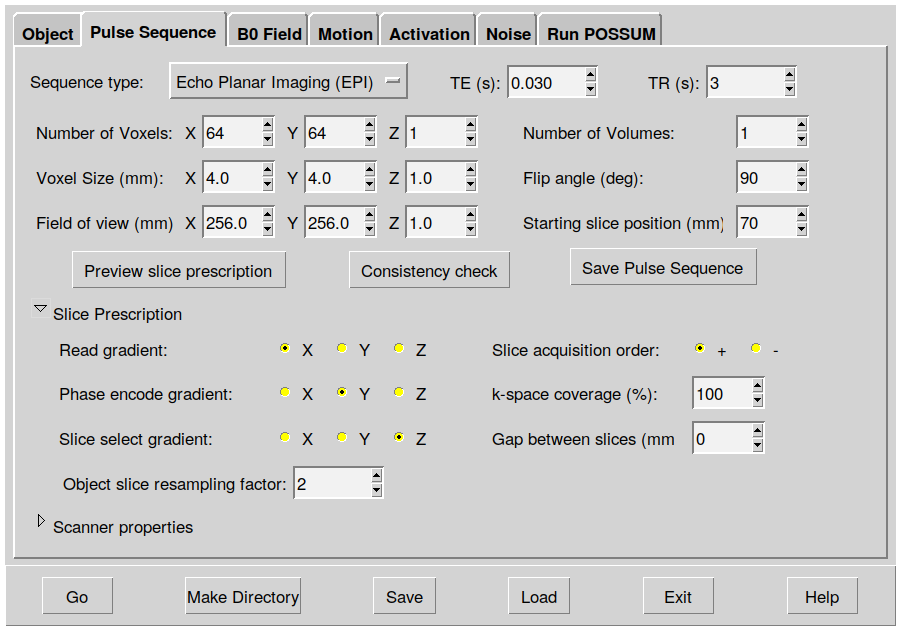
\includegraphics[width=.6\textwidth]{7/possum-gui.png}
\caption{The ``Pulse Sequence'' specifications page in the POSSUM GUI}
\label{fig:possum}
\end{figure}

The biggest drawback to POSSUM is the degree of MR physics knowledge needed to use it effectively. For MR physicists, specifying the details of a pulse sequence may be trivial. For researchers from other fields, customizing pulse sequence parameters, an example of which can be seen in Figure \ref{fig:possum}, can be a challenging task. These customizations may even be unnecessary depending on the goals a researcher hopes to achieve using the simulated data.

If a researcher's goal is to test the impact of a new MRI processing technique on known signals in an image, the BrainWeb MRI simulator might be a better option than POSSUM. BrainWeb was created and is actively developed by the \href{mcgill.ca/bic/}{McConnell Brain Imaging Centre} at McGill University to assist in validation computer-aided MRI analysis tools \cite{kwan1999mri} \cite{collins1998design} \cite{cocosco1997brainweb} \cite{kwan1996extensible}. A set of simulated images have been generated using BrainWeb and are can be found in the BrainWeb Simulated Brain Database (SBD). The SBD contains simulated images for healthy subjects and for subjects who have lesions due to multiple sclerosis.

Custom simulations can be generated on the BrainWeb server by submitting a request via a browser. The simulation request form has three areas which can be customized: the type of brain to simulate, the MR pulse sequence, and the imaging artifacts. The simulation is run on the server and the user is notified via email when the simulated images are ready to download. 

BrainWeb's simulator is slightly more approachable than POSSUM: a limited number of pulse sequence parameters are available to customize and a description is listed next to each parameter in the pulse sequence and imaging artifacts sections. However, the user has slightly less control over the simulated image. The brain models used by BrainWeb are healthy brains or brains with MS lesions. It is not an option for the user to upload an image to use as the structural information in the sequence. For our purposes, the biggest limitation of BrainWeb is that it only simulates structural images. 

Our simulation tool, SPECTr, is one of the few tools which simulates resting-state fMRIs. It offers the opportunity for researchers to explore the effects of their motion correction techniques on BOLD signal, background noise, and patient motion using a lightweight simulation that can be run on a personal computer. It should be noted that SPECTr is not a substitute for the physics-based models in POSSUM and BrainWeb: it is intended to evaluate signal changes in rs-fMRI sequences as a result of post-acquisition image processing.

\subsection{Volume Registration} 

To the best of our knowledge, the only other study that has used a variant of the DAG-based method was performed by Liao et al \cite{Liao2016}. Liao et al’s dataset consisted of 10 fetal rs-fMRIs. In each of these sequences, the fetal brain, fetal liver, and placenta were manually segmented in the first volume of the sequence as well as in five other randomly chosen volumes. These overlap of these manual segmentations before and after registration as measured using the Dice coefficient was used to quantify the amount of motion in each sequence. Even though the Dice coefficients increase more in each sequence after Liao et al.’s registration than after traditional registration, their measure of positional change fails to quantify any changes in position between any other pairs of volumes that do not have manual segmentations. 

The fetal images used in Liao et al.'s study included images of singleton, twin, and triplet pregnancies. There is significant potential value in the study of fetal motion in multifetal pregnancies. Considering the motion patterns alone, it would be expected that the singleton pregnancies have different motion patterns than the multifetal pregnancies

\subsection{Age Group Specific Motion}

It has been established that motion is often correlated with patient age in adolescent population. Satterthwaite et al. specifically designed an imaging study of adolescents ages 8-23 such that patient age and motion were uncorrelated \cite{Satterthwaite2012} % ELEPHANTS check citation
In our study, patient age was described only as fetal, neonatal, or preadolescent despite a range of ages in each group. We establish that there are characteristics of patient motion specific to each group, but we did not consider more granular ranges of patient age. Additional analyses would need to be considered to determine whether post-conceptual age for fetal and neonatal subjects impacts motion characteristics. 

In the fetal cohort, it is possible that there are motion characteristics linked to post-conceptual age. As a fetus grows, the amount of room in the uterus in which it can move decreases. However, as the fetal brain develops, the fetus may begin to move in different ways to test its biological systems. 

Studies involving neonatal cohorts often track two ages for the subjects: the post-conceptual age and the age since birth. The relationship between these two ages and a neonate's brain development could impact the amount of motion exhibited during a scan.